%%%%%%%%%%%%%%%%%%%%%%%%%%%%%%%%%%%%%%%%%
% Short Sectioned Assignment
% LaTeX Template
% Version 1.0 (5/5/12)
%
% This template has been downloaded from:
% http://www.LaTeXTemplates.com
%
% Original author:
% Frits Wenneker (http://www.howtotex.com)
%
% License:
% CC BY-NC-SA 3.0 (http://creativecommons.org/licenses/by-nc-sa/3.0/)
%
%%%%%%%%%%%%%%%%%%%%%%%%%%%%%%%%%%%%%%%%%

%----------------------------------------------------------------------------------------
%	PACKAGES AND OTHER DOCUMENT CONFIGURATIONS
%----------------------------------------------------------------------------------------

\documentclass[paper=a4, fontsize=11pt]{scrartcl} % A4 paper and 11pt font size

\usepackage[T1]{fontenc} % Use 8-bit encoding that has 256 glyphs
\usepackage{fourier} % Use the Adobe Utopia font for the document - comment this line to return to the LaTeX default
\usepackage[english]{babel} % English language/hyphenation
\usepackage{amsmath,amsfonts,amsthm, amssymb} % Math packages
\usepackage{enumitem}
\usepackage{cancel}
\usepackage{graphicx} % Required to insert images
\usepackage{color}
\definecolor{dkgreen}{rgb}{0,0.6,0}
\definecolor{gray}{rgb}{0.5,0.5,0.5}
\definecolor{mauve}{rgb}{0.58,0,0.82}
\usepackage{listings}
\lstset{frame=tb,
  language=Python,
  aboveskip=3mm,
  belowskip=3mm,
  showstringspaces=false,
  columns=flexible,
  basicstyle={\small\ttfamily},
  numbers=none,
  numberstyle=\tiny\color{gray},
  keywordstyle=\color{blue},
  commentstyle=\color{dkgreen},
  stringstyle=\color{mauve},
  breaklines=true,
  breakatwhitespace=true
  tabsize=3
}
\usepackage{pgfplotstable}% For inserting csv table

\usepackage{sectsty} % Allows customizing section commands
\allsectionsfont{\centering \normalfont\scshape} % Make all sections centered, the default font and small caps

\usepackage{fancyhdr} % Custom headers and footers
\pagestyle{fancyplain} % Makes all pages in the document conform to the custom headers and footers
\fancyhead{} % No page header - if you want one, create it in the same way as the footers below
\fancyfoot[L]{} % Empty left footer
\fancyfoot[C]{} % Empty center footer
\fancyfoot[R]{\thepage} % Page numbering for right footer
\renewcommand{\headrulewidth}{0pt} % Remove header underlines
\renewcommand{\footrulewidth}{0pt} % Remove footer underlines
\setlength{\headheight}{13.6pt} % Customize the height of the header

\numberwithin{equation}{section} % Number equations within sections (i.e. 1.1, 1.2, 2.1, 2.2 instead of 1, 2, 3, 4)
\numberwithin{figure}{section} % Number figures within sections (i.e. 1.1, 1.2, 2.1, 2.2 instead of 1, 2, 3, 4)
\numberwithin{table}{section} % Number tables within sections (i.e. 1.1, 1.2, 2.1, 2.2 instead of 1, 2, 3, 4)

\setlength\parindent{0pt} % Removes all indentation from paragraphs - comment this line for an assignment with lots of text

%----------------------------------------------------------------------------------------
%	TITLE SECTION
%----------------------------------------------------------------------------------------

\newcommand{\horrule}[1]{\rule{\linewidth}{#1}} % Create horizontal rule command with 1 argument of height

\title{	
\normalfont \normalsize 
\textsc{Baruch, MFE} \\ [25pt] % Your university, school and/or department name(s)
\horrule{0.5pt} \\[0.4cm] % Thin top horizontal rule
\huge MTH 9876 Assignment Four\\  % The assignment title
\horrule{2pt} \\[0.5cm] % Thick bottom horizontal rule
}


\author{Zhou, ShengQuan} % Your name

\date{\normalsize\today} % Today's date or a custom date

\begin{document}
	


\maketitle % Print the title

\newpage



\section{Marshall-Olkin Copula}
Consider the Marshall-Olkin copula $C_{\text{MO}}(u_1,u_2)$.\\

\textbf{(i)} Calculate the Spearman's rho of $C_{\text{MO}}(u_1,u_2)$.\\
\textit{Solution}: According to lecture notes,
$$
C_{\text{MO}}(u_1,u_2) = u_1 u_2\min\left( u_1^{-\alpha_1}, u_2^{-\alpha_2} \right)
= \min\left( u_1^{1-\alpha_1}u_2, u_1 u_2^{1-\alpha_2} \right),
$$
where $\alpha_1 = \frac{\lambda_{12}}{\lambda_1 +\lambda_{12}}$ and $\alpha_2 = \frac{\lambda_{12}}{\lambda_2 +\lambda_{12}}$. \textbf{Note}: there is
a typo in lecture notes for $\alpha_1$ and $\alpha_2$.\\

Notice that
the two arguments of the $\min$ function are equal when
$$
u_1^{-\alpha_1} = u_2^{-\alpha_2} \Rightarrow u_2 = u_1^{\frac{\alpha_1}{\alpha_2}}.
$$

The Spearman's rho is given by
$
\rho_S(X,Y) = 12\int\int_{[0,1]^2} C(u_1,u_2)du_1 du_2 - 3
$, where we calculate the integral in two sub-regions of $(u_1,u_2)\in [0,1]^2$ separated by the line $u_1^{-\alpha_1} = u_2^{-\alpha_2}$.
\begin{align*}
\int\int_{[0,1]^2} C(u_1,u_2)du_1 du_2 &= \int\int_{u_1^{-\alpha_1} > u_2^{-\alpha_2}} u_1 u_2^{1-\alpha_2 }du_1 du_2
+ \int\int_{u_1^{-\alpha_1} < u_2^{-\alpha_2}} u_1^{1-\alpha_1} u_2 du_1 du_2 \\
 &= \int_0^1 du_1 u_1\int_{u_1^{\alpha_1/\alpha_2}}^1 du_2  u_2^{1-\alpha_2 }
+ \int_0^1 du_1 u_1^{1-\alpha_1}\int_0^{u_1^{\alpha_1/\alpha_2}}  u_2 du_2\\
&= \frac{1}{2-\alpha_2} \int_0^1 du_1 u_1 \left[ 1- u_1^{\frac{\alpha_1}{\alpha_2} (2-\alpha_2)} \right]
+ \frac{1}{2}\int_0^1 du_1 u_1^{1-\alpha_1 + 2\frac{\alpha_1}{\alpha_2}}\\
&= \frac{1}{2-\alpha_2}\int_0^1 u_1 du_1  + \left(\frac{1}{2} - \frac{1}{2-\alpha_2}\right)\int_0^1 du_1 u_1^{1-\alpha_1 + 2\frac{\alpha_1}{\alpha_2}}\\
&= \frac{1}{2(2-\alpha_2)} + \left(\frac{1}{2} - \frac{1}{2-\alpha_2}\right)\frac{1}{2-\alpha_1 + 2\frac{\alpha_1}{\alpha_2}}\\
&= \frac{2\alpha_1+2\alpha_2-\alpha_1\alpha_2 -\alpha_2^2}{2(2-\alpha_2)(2\alpha_1 + 2\alpha_2 -\alpha_1\alpha_2)}\\
&= \frac{\alpha_1  + \alpha_2}{2(2\alpha_1 + 2\alpha_2 -\alpha_1\alpha_2)}.
\end{align*}
Thus,
$$
\rho_S(X,Y) = 12 \times \frac{\alpha_1  + \alpha_2}{2(2\alpha_1 + 2\alpha_2 -\alpha_1\alpha_2)} -3 = 
\frac{3\alpha_1 \alpha_2}{2\alpha_1 + 2\alpha_2 -\alpha_1\alpha_2} = \frac{3\lambda_{12}^2}{2\lambda_1\lambda_{12} + 2\lambda_2\lambda_{12} + 3\lambda_{12}^2}.
$$
\newpage

\textbf{(ii)} Calculate the limits $\lambda_U$ and $\lambda_L$ and determine whether the
Marshall-Olkin copula has upper and/or lower tail dependence.\\
\textit{Solution}: Set $u_1 = u_2 = u$,
$
C(u,u) = u^{2-\min(\alpha_1,\alpha_2)}
$. Thus, the upper tail dependence
\begin{align*}
\lambda_U &\triangleq \lim_{u\rightarrow 1}\frac{1-2u + C(u,u)}{1-u}\\
&= \lim_{u\rightarrow 1}\frac{1-2u + u^{2-\min(\alpha_1,\alpha_2)}}{1-u}\\
(v\triangleq 1-u) &= \lim_{v \rightarrow 0}\frac{2v-1 + (1-v)^{2-\min(\alpha_1,\alpha_2)}}{v}\\
&= \lim_{v \rightarrow 0}\frac{2v-1 + 1 -\left(2-\min(\alpha_1,\alpha_2)\right)v}{v}\\
&= \min(\alpha_1,\alpha_2).
\end{align*}
The lower tail dependence
\begin{align*}
\lambda_L &\triangleq \lim_{u\rightarrow 0}\frac{C(u,u)}{u}\\
&= \lim_{u\rightarrow 0}\frac{u^{2-\min(\alpha_1,\alpha_2)}}{u}\\
&= \lim_{u\rightarrow 0}u^{1-\min(\alpha_1,\alpha_2)}\\
&= 0.
\end{align*}
The last equality results from the fact that $\alpha_1\le 1$ and $\alpha_2 \le 1$.\\

\textbf{(iii)} Propose a simulation algorithm for $C_{\text{MO}}(u_1,u_2)$. Choose
$\lambda_1 = 1.7, \lambda_2 = 0.7, \lambda_{12} = 0.3$, and generate 2000 samples from
$C_{\text{MO}}(u_1,u_2)$. Plot the results in a $1\times 1$-square.\\
\textit{Solution}: The sampling algorithm is constructed as follows:
\begin{itemize}[noitemsep]
\item Generate independent exponentially distributed random numbers $T_1, T_2, T_{12}$ with intensities $\lambda_1, \lambda_2, \lambda_{12}$
respectively. This is because $T_1, T_2, T_{12}$ are arriving times of independent Poisson processes. The marginal 
distributions of the survival probabilities are
$$
\mathbb{P}(T_i>t) = e^{-\lambda_i t}, \quad i=1,2,12.
$$
\item Take $\tau_1=\min(T_1,T_{12})$ and $\tau_2 = \min(T_2,T_{12})$. The marginal distributions of the survival probabilities are
$$
F_i(t)\triangleq \mathbb{P}(\tau_i>t) = e^{-(\lambda_i + \lambda_{12}) t}, \quad i=1,2.
$$
\item By definition, $U_i = F_i(\tau_i) = e^{-(\lambda_i + \lambda_{12}) \tau_i}$, $i=1,2$.\\
\end{itemize}
Python script:
\begin{lstlisting}
import math
import numpy as np
import matplotlib.pyplot as plt
lambda1=1.7
lambda2=0.7
lambda12=0.3
ns=2000

T1  = np.random.exponential(1.0/lambda1,  ns)
T2  = np.random.exponential(1.0/lambda2,  ns)
T12 = np.random.exponential(1.0/lambda12, ns)

tau1 = np.minimum(T1, T12)
tau2 = np.minimum(T2, T12)

u1 = np.exp(-(lambda1+lambda12)*tau1)
u2 = np.exp(-(lambda2+lambda12)*tau2)

plt.xlabel("u1")
plt.ylabel("u2")
plt.show()
\end{lstlisting}
\begin{figure}[h]\label{survival}
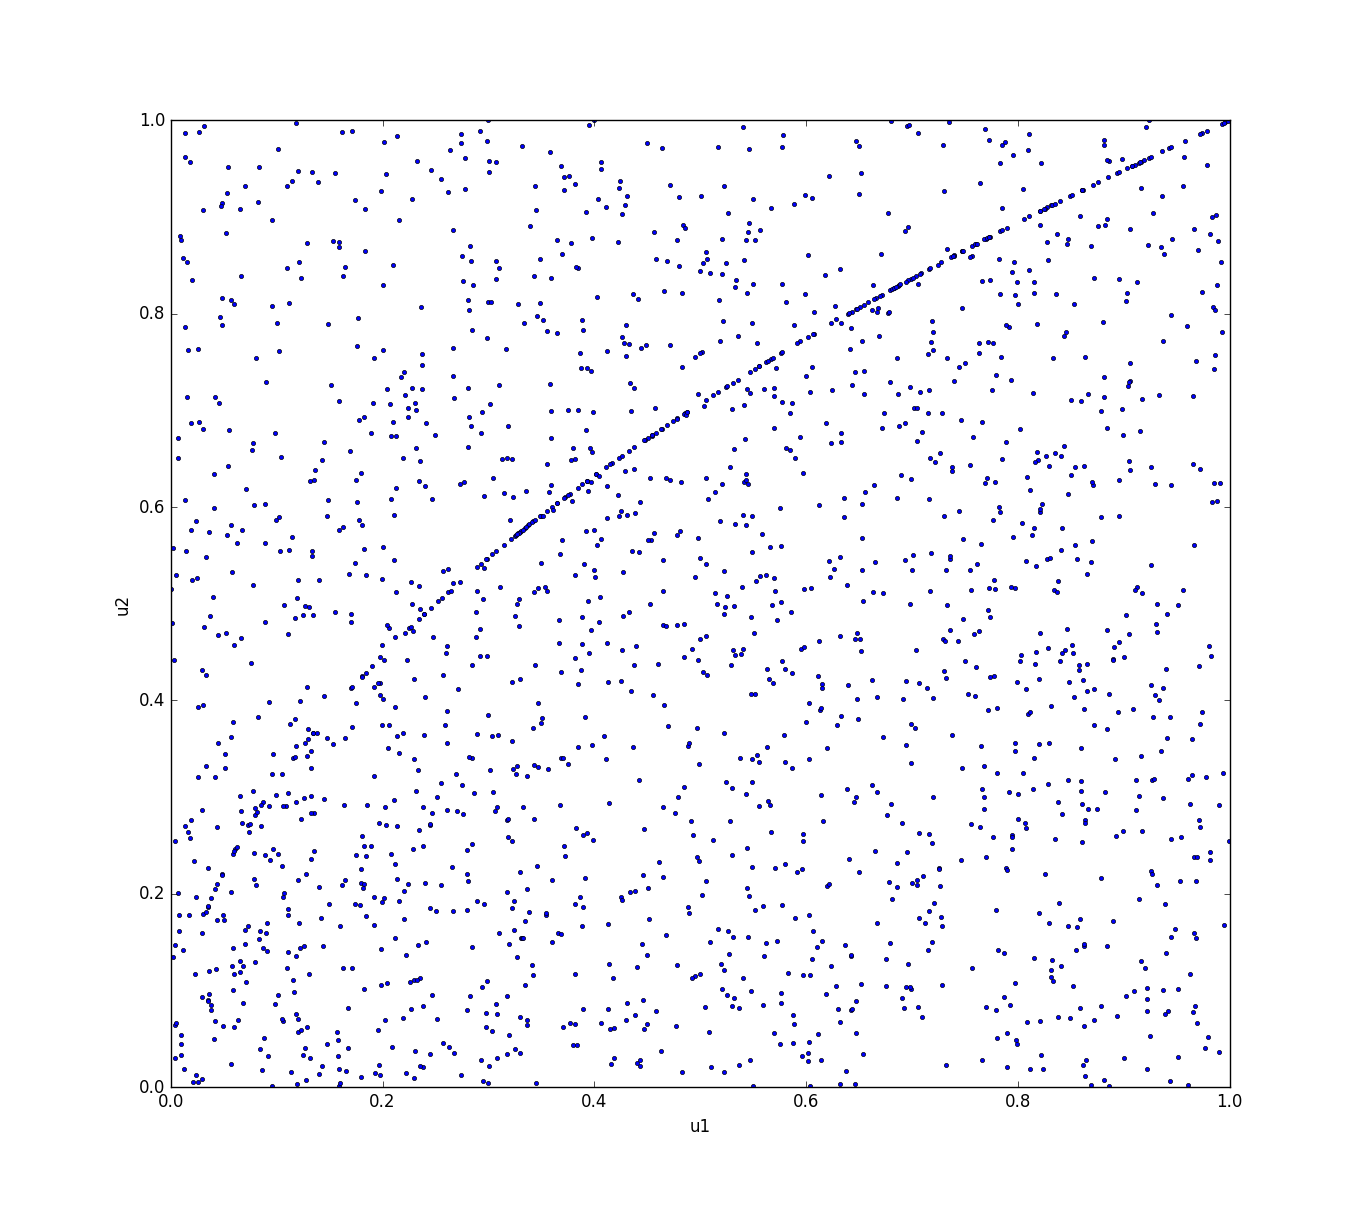
\includegraphics[width=14cm]{mo}
\end{figure}

\newpage
\section{Two-Factor Gaussian Copula Model}
Consider the following two-factor generalization of the one-factor Gaussian copula model:
$$
Z_i = \beta_{i1}S_1 + \beta_{i2}S_2 + \sqrt{1 - \beta_{i1}^2 - \beta_{i2}^2}\epsilon_i,
$$
where $S_1,S_2\sim N(0,1)$ are independent, $\beta_{i1}^2 + \beta_{i2}^2 < 1$, for each
$i=1,\cdots,N$, and $\epsilon_i \sim N(0,1)$ are independent of $S_1$ and $S_2$.\\

\textbf{(i)} Determine the correlation structure in this model.\\
\textit{Solution}: For $i=1,\cdots,N$, $\mathbb{E}[Z_i] = 0$. For $i,j=1,\cdots,N$,
\begin{align*}
\mathbb{E}\left[Z_i Z_j\right] &= \mathbb{E}\left[ \left(\beta_{i1}S_1 + \beta_{i2}S_2 + \sqrt{1 - \beta_{i1}^2 - \beta_{i2}^2}\epsilon_i\right)
\left(\beta_{j1}S_1 + \beta_{j2}S_2 + \sqrt{1 - \beta_{j1}^2 - \beta_{j2}^2}\epsilon_j\right) \right]\\
&= \beta_{i1}\beta_{j1}+ \beta_{i2}\beta_{j2} + \sqrt{\left( 1 - \beta_{i1}^2 - \beta_{i2}^2 \right)\left( 1 - \beta_{j1}^2 - \beta_{j2}^2 \right)}\delta_{ij}.
\end{align*}
In other words,
\begin{align*}
\rho_{ij} = \begin{cases}
\beta_{i1}\beta_{j1}+ \beta_{i2}\beta_{j2}, \quad & i\neq j,\\
1, \quad &i=j.
\end{cases}
\end{align*}

\textbf{(ii)} Derive, along the lines of the calculations done in class for the one-factor
model, the LHP limit of this model.\\
\textit{Solution}: The \textit{homogeneous} part of LHP assumption, $\beta_{i1}=\beta_1$, $\beta_{i2}=\beta_2$, identical LGDs $l_i = l$, and 
identical default probabilities $Q_i(T)=Q(T)$, $\forall i=1,\cdots,N$. 
The conditional loss distribution
\begin{align*}
\mathbb{P}\left(  L_N(T) = kl |S_1 = s_1, S_2 = s_2\right)
= \begin{pmatrix}
N\\ k
\end{pmatrix} Q(T|s_1,s_2)^k \left( 1- Q(T|s_1,s_2) \right)^{N-k},
\end{align*}
where $Q(T|s_1,s_2)$ is the default probability by time $T$, conditioned on the two driving factors $S_1=s_1, S_2=s_2$,
\begin{align*}
Q(T|s_1,s_2) &\triangleq Q(T|S_1=s_1,S_2=s_2)\\
&= \mathbb{P}(\tau_i \le T|S_1=s_1,S_2=s_2)\\
&= \mathbb{P}( Z_i \le H_i(T) |S_1=s_1,S_2=s_2), \quad H_i(t) \triangleq N^{-1}(Q_i(t))\\
&= \mathbb{P}\left( \beta_1 S_1 + \beta_2 S_2 + \sqrt{1-\beta_1^2 - \beta_2^2}\epsilon_i \le H_i(T) \bigg|S_1=s_1,S_2=s_2\right)\\
&= \mathbb{P}\left( \beta_1 s_1 + \beta_2 s_2 + \sqrt{1-\beta_1^2 - \beta_2^2}\epsilon_i \le H_i(T)\right)\\
&= \mathbb{P}\left(  \epsilon_i \le \frac{H_i(T) - \beta_1 s_1 - \beta_2 s_2}{\sqrt{1-\beta_1^2 - \beta_2^2}}\right)\\
&= N\left( \frac{H(T) - \beta_1 s_1 - \beta_2 s_2}{\sqrt{1-\beta_1^2 - \beta_2^2}} \right), \quad  H(t) \triangleq N^{-1}(Q(t)).
\end{align*}\\

The total loss distribution
\begin{align*}
\mathbb{P}\left(  L_N(T) = kl \right)
&= \frac{1}{2\pi}\int_{-\infty}^{-\infty}\int_{-\infty}^{-\infty} \mathbb{P}\left(  L_N(T) = kl |S_1 = s_1, S_2 = s_2\right)
e^{-\frac{s_1^2+s_2^2}{2}} ds_1 ds_2.
\end{align*}\\

The \textit{large} part of LHP assumption, $N\rightarrow \infty$, let $l_N =\frac{L(T)}{N}$ denote the number
of defaulting names per portfolio size. According to lecture notes,
\begin{align*}
\mathbb{E}[l_N|s_1,s_2] &= l Q(T|s_1,s_2)\\
\text{Var}[l_N|s_1,s_2] &= \frac{l^2}{N} Q(T|s_1,s_2) (1-Q(T|s_1,s_2))\rightarrow 0.
\end{align*}
The above result indicates that in the large portfolio limit $N\rightarrow \infty$, $l_N =\frac{L(T)}{N}$
is non-random when conditioned on $S_1=s_1,S_2=s_2$. In other words, all the randomness comes from the two driving
factor $S_1$ and $S_2$. Thus, replacing the conditional value $s_1$ and $s_2$ by the random variables $S_1$ and $S_2$,
\begin{align*}
\mathbb{P}\left( l_{\infty} \le xl \right) &= \mathbb{P}\left( Q(T|S_1,S_2) \le x \right)\\
&=  \mathbb{P}\left( Q(T|S_1,S_2) \le x \right) \\
&=  \mathbb{P}\left( N\left( \frac{H(T) - \beta_1 S_1 - \beta_2 S_2}{\sqrt{1-\beta_1^2 - \beta_2^2}} \right)  \le x \right) \\
&=  \mathbb{P}\left( \frac{H(T) - \beta_1 S_1 - \beta_2 S_2}{\sqrt{1-\beta_1^2 - \beta_2^2}}  \le N^{-1}(x) \right) \\
&=  \mathbb{P}\left( \beta_1 S_1 + \beta_2 S_2 \le H(T) - \sqrt{1-\beta_1^2 - \beta_2^2}N^{-1}(x) \right).
\end{align*}
Since $\beta_1 S_1 + \beta_2 S_2 \sim N\left(0,\beta_1^2+\beta_2^2\right)$,
$$
\mathbb{P}\left( l_{\infty} \le xl \right) = N\left( \frac{H(T) - \sqrt{1-\beta_1^2 - \beta_2^2}N^{-1}(x) }{\sqrt{\beta_1^2+\beta_2^2}}\right).
$$

\newpage

\section{Historical Simulation of VaR}
Assume that the CCP calculates the margin requirements by means of VaR
at the $p = 99\%$ confidence level. Regulatory authorities require that the
CCP back-test the performance of its risk model by calculating the number
of breaches of the VaR model over the test period of the most recent 250
days (one year). Specifically, on each day of the test period, the daily 
portfolio loss (in reality, it is the $n$-day portfolio loss, where $n$ 
is called the market period of risk (MPOR)) 
is compared to the calculated VaR level. A VaR breach means
that the loss on a given day exceeds the VaR level.\\

\textbf{(i)} Assuming that the daily portfolio returns are independent of each other,
find the probability distribution of the number of VaR breaches. What
is the expected number of VaR breaches?\\
\textit{Solution}: Setting the confidence level at $p = 99\%$ means empirically, one
out of 100 sample returns is a VaR breach. Assuming that the daily portfolio returns 
are independent of each other, find the probability distribution of the number of VaR 
breaches is
$$
 \mathbb{P}(\text{\# of VaR breaches} = k ) = \begin{pmatrix}
250\\ k
\end{pmatrix}  0.01^k 0.99^{250-k}.
$$
The expected number of VaR breaches is $250\times 0.01 = 2.5$.\\

\textbf{(ii)} Determine numerically the probability of $k = 0, 1, \cdots, 10$ VaR breaches.\\
\textit{Solution}: Tabulated below. The first row records $ \mathbb{P}(\text{\# of VaR breaches} = k )$
and the second row records $\mathbb{P}(\text{\# of VaR breaches} \ge k )$.
\begin{center}
\footnotesize{
\begin{tabular}{l*{11}{c}r}
\hline
$k$              & 0 & 1 & 2 & 3 & 4  & 5 & 6 & 7 & 8 & 9 & 10 \\
\hline
$\mathbb{P}(=k )$ & 0.0811 & 0.2047 & 0.2574 & 0.2149 & 0.1341 & 0.0666 & 0.0273 & 0.0097 & 0.0030 & 0.0008 & 0.0002 \\
\hline
$\mathbb{P}(\ge k )$ & 0.0811 & 0.2858 & 0.5432 & 0.7581 & 0.8922 & 0.9588 & 0.9861 & 0.9958 & 0.9988 & 0.9996 & 0.9998 \\
\hline
\end{tabular}
}\\
\end{center}


\textbf{(iii)} Portfolio back test showed 4 VaR breaches. Can one reject, at the
confidence level of $95\%$, the hypothesis that the VaR model is working
properly?\\
\textit{Solution}: From the second row of the above table,
$$
\mathbb{P}(\text{\# of VaR breaches} \ge 5 ) < 5\%.
$$
In other words, given a number of 4 VaR breaches, the hypothesis that the VaR model is working
properly cannot be rejected at the
confidence level of $95\%$.

\end{document}